%!TEX root = ../main.tex
\section{Additional Experiments}
\label{sec:app-add-experiments}

\textbf{Comparison between REINFORCE and GPOMDP \cite{baxter01jair-gpomdp}.} In the main text, we focused on the vanilla REINFORCE estimator. We also conducted experiments with the GPOMDP estimator, which replaces the full trajectory return with reward-to-go terms using the Markov property. GPOMDP can have lower variance than REINFORCE \cite{papini22ml-reinforcevariance}. The same moment-evaluation framework can be directly applied to these cases by changing the return $R(\tau)$ to running return $G_t$ which is still a quadratic function of the underlying Gaussian variables. We find that the NSR landscape is qualitatively similar to the REINFORCE case, with the same trend of increasing NSR near optimality. (Figure~\ref{fig:gpomdp}).

\begin{figure}
    \centering
    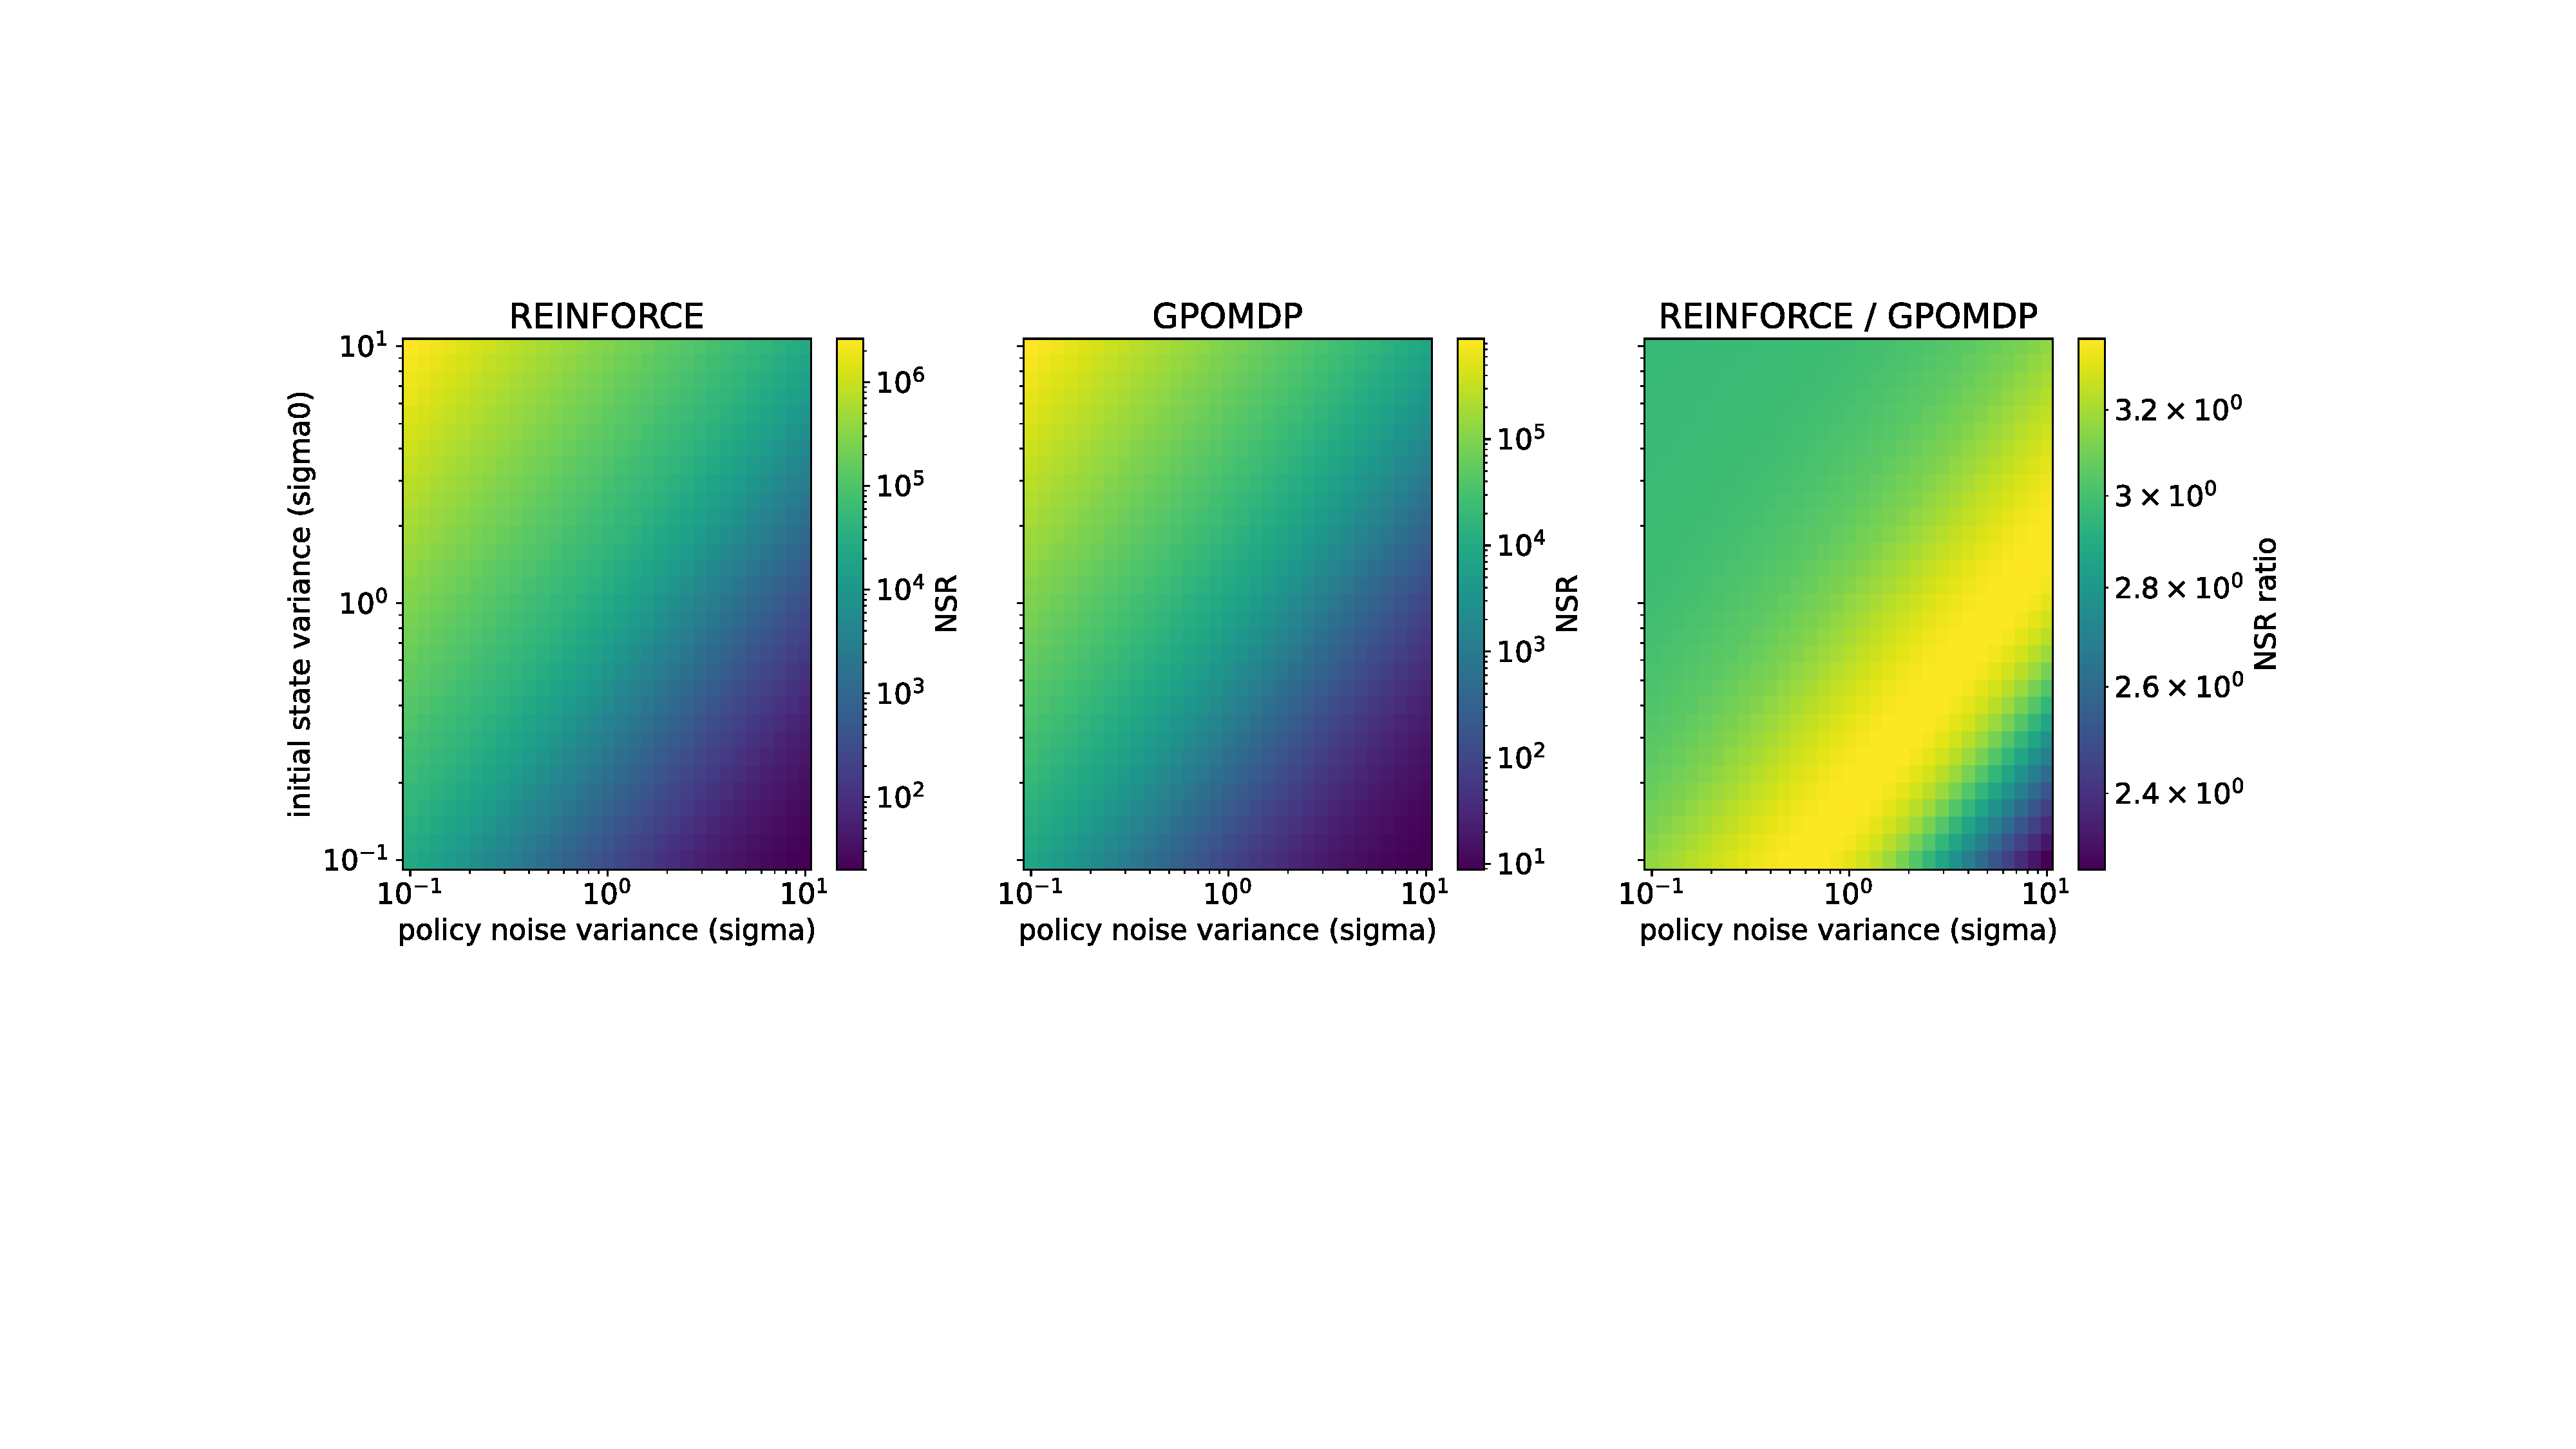
\includegraphics[width=0.9\textwidth]{figure/gpomdp.pdf}
    \caption{NSR landscape for REINFORCE, GPOMDP and their ratio. The NSR landscape for GPOMDP is qualitatively similar to that of REINFORCE, with the same trend of increasing NSR near optimality.}
    \label{fig:gpomdp}
\end{figure}

\textbf{Monte Carlo estimation of NSR.}
We empirically investigate the accuracy of Monte Carlo estimation of the variance and the NSR. Our results show that Monte Carlo estimates fail to accurately capture the trends of both the variance and the NSR along optimization trajectories, even when using a large number of rollouts (Figure~\ref{fig:mc_nsr}). This highlights the value of exact characterizations of the REINFORCE variance and the NSR, which can further enable rigorous analyses of policy-gradient optimization dynamics.

\begin{figure}
    \centering
    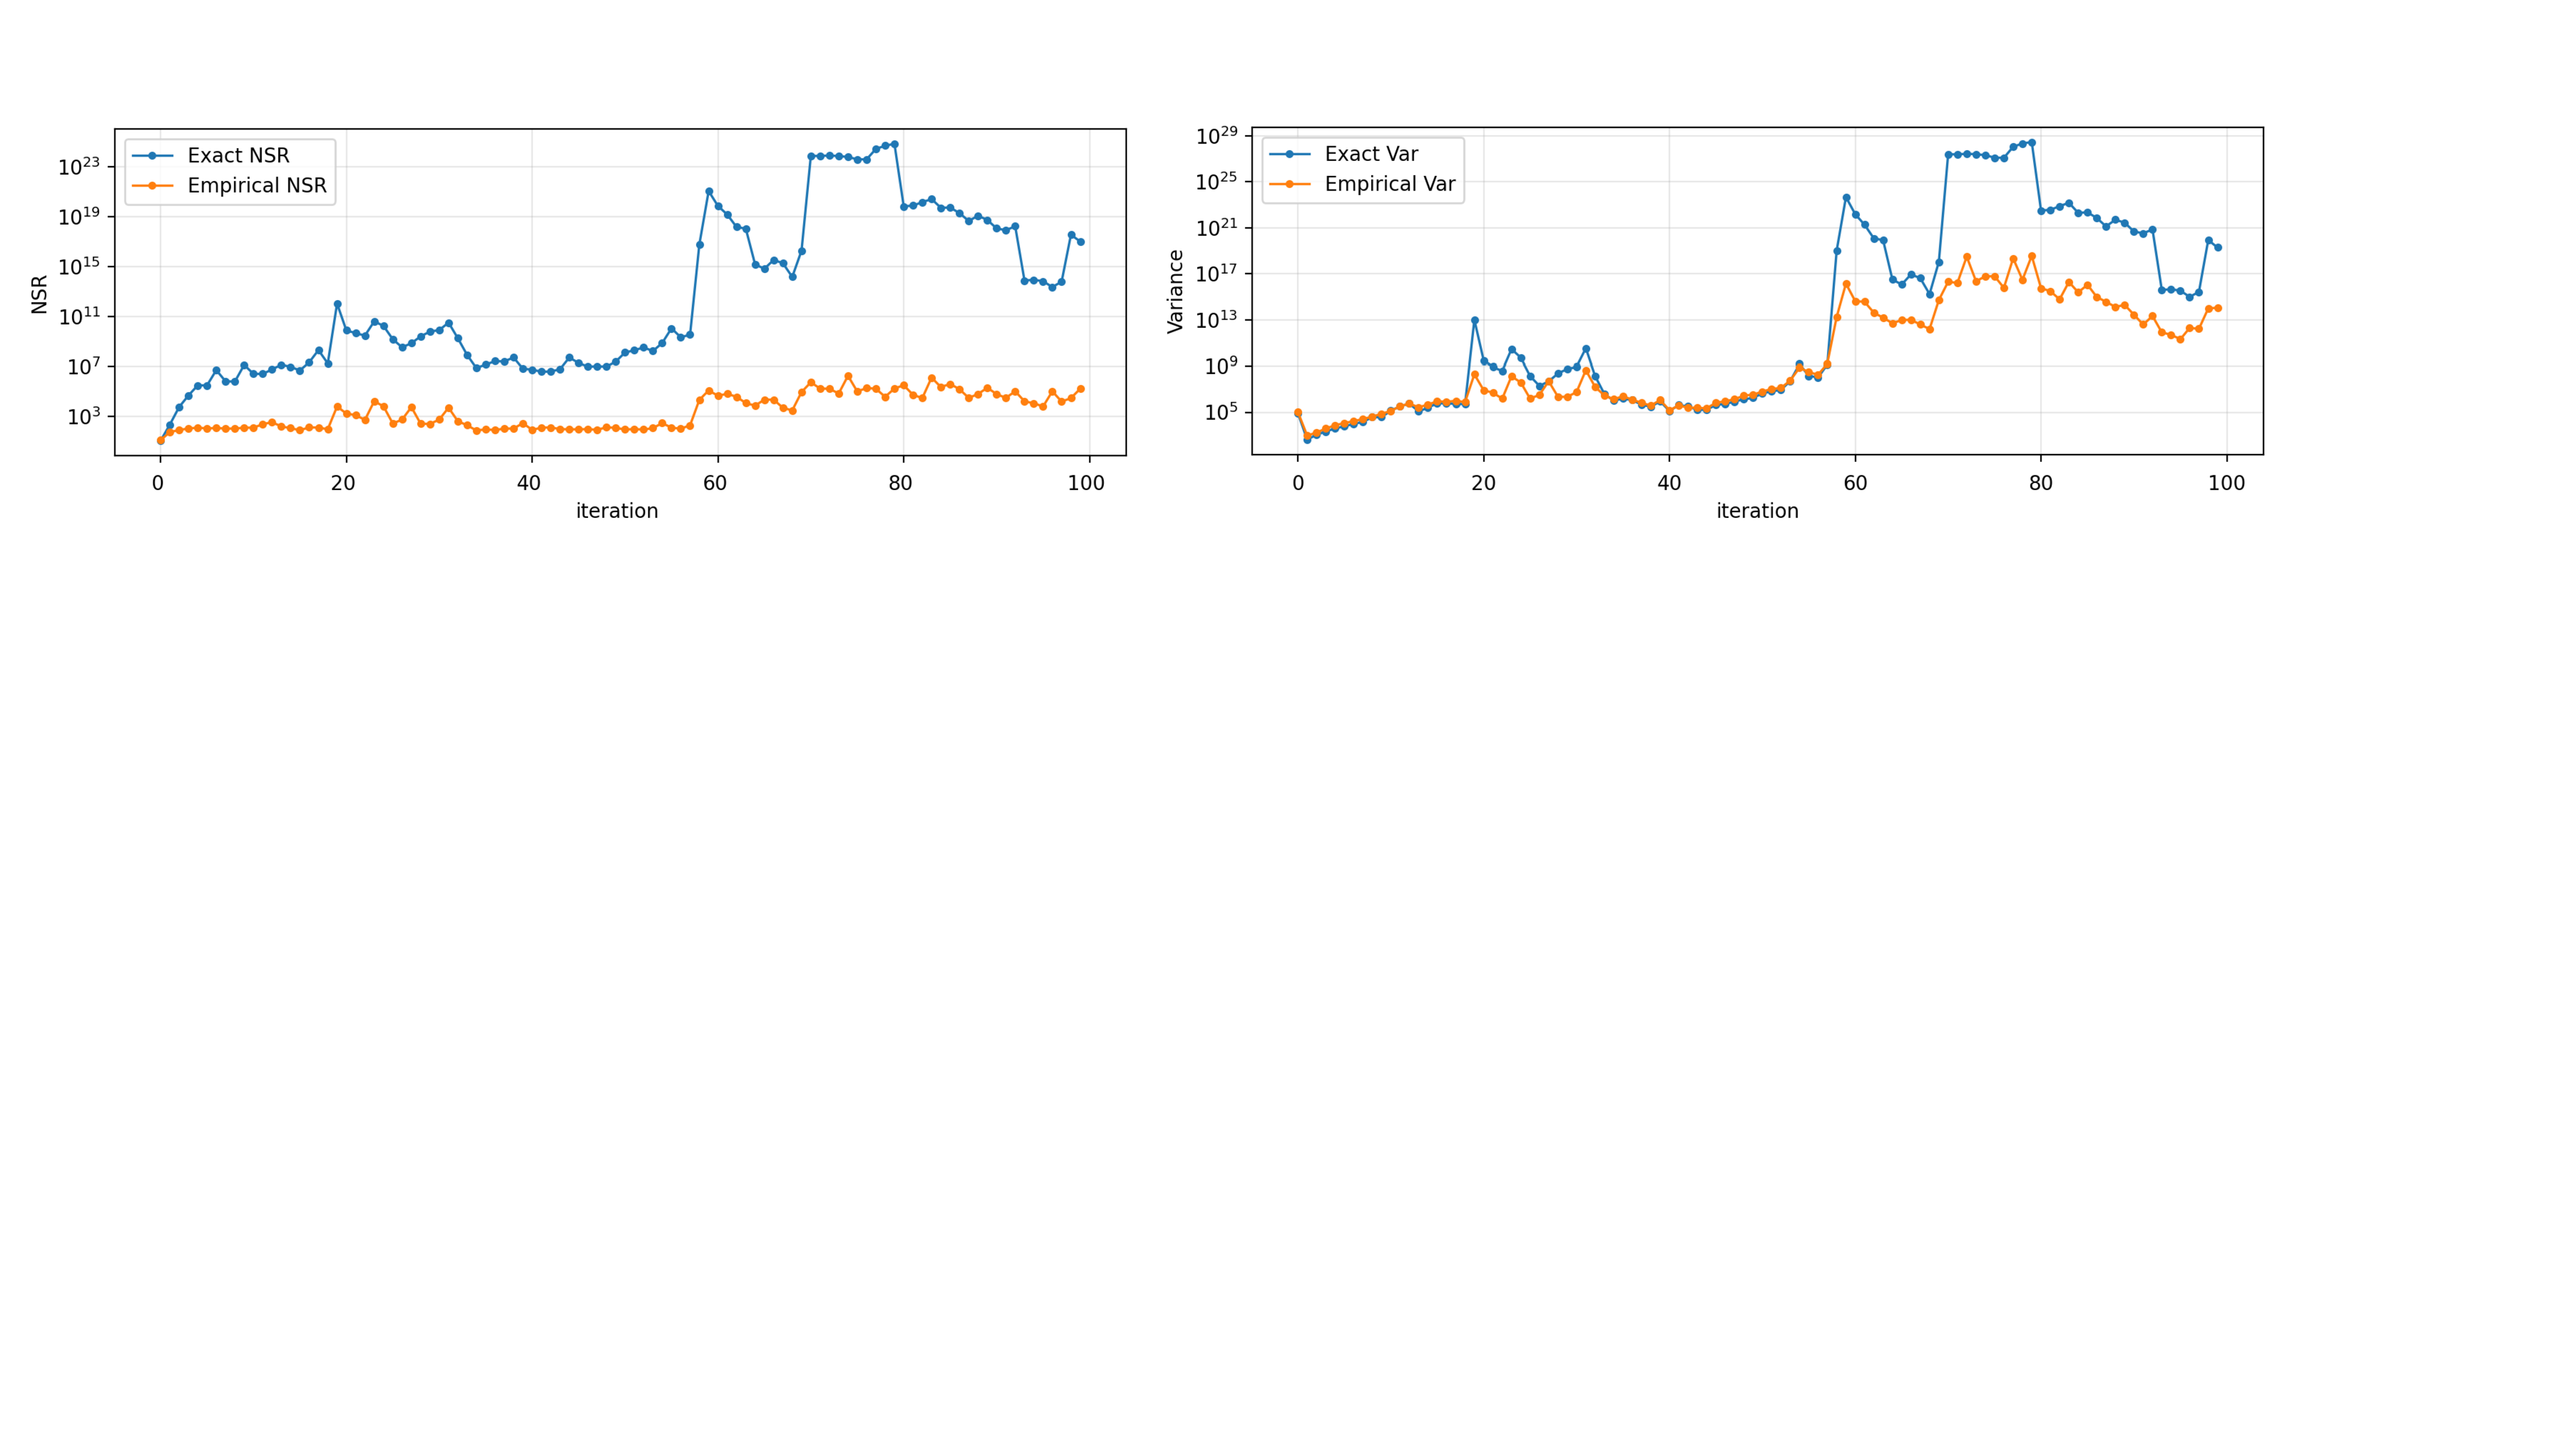
\includegraphics[width=0.9\textwidth]{figure/mc_nsr.pdf}
    \caption{Monte Carlo estimation of the NSR. Orange line: empirical Monte Carlo estimate with 10 minutes limit each iteration. Blue line: exact NSR. Even with a large number of rollouts, the empirical Monte Carlo estimate fails to accurately capture the trends of the variance and the NSR along optimization trajectories.}
    \label{fig:mc_nsr}
\end{figure}

\textbf{Experiment details.}
For all experiments below, we set the initial exploration covariance to $\Sigma_0 = I$. In the multi-step LQG experiments with double-integrator dynamics, we use Adam with learning rate $10^{-3}$, SGD with learning rate $10^{-4}$, and batch size $2^{10}$. In the polynomial-system experiments, we use the same learning rates for Adam and SGD, with batch size $2^{12}$. For the policy-collapse experiments on the quadratic system, we use Adam with learning rate $10^{-2}$ and batch size $2^6$. For the experiments with nonlinear dynamics and MLP policies, we use two-layer MLPs with 64 hidden units and ReLU activations, Adam with learning rate $10^{-2}$, and batch size $2^{12}$. The NSR and variance for the nonlinear dynamics experiments are estimated via Monte Carlo with 1 minute limit per iteration.

\textbf{Additional MuJoCo experiments.} In addition to the pendulum/LQR with MLP policy and polynomial system experiments in the main text, we also conducted experiments on the MuJoCo Hopper and HalfCheetah environments with MLP policies. We train these policies using PPO. We observe coupled fluctuations between NSR and objective value, suggesting that high-NSR regimes are associated with instability in policy optimization (Figure~\ref{fig:mujoco_collapse}).

\begin{figure}
    \centering
    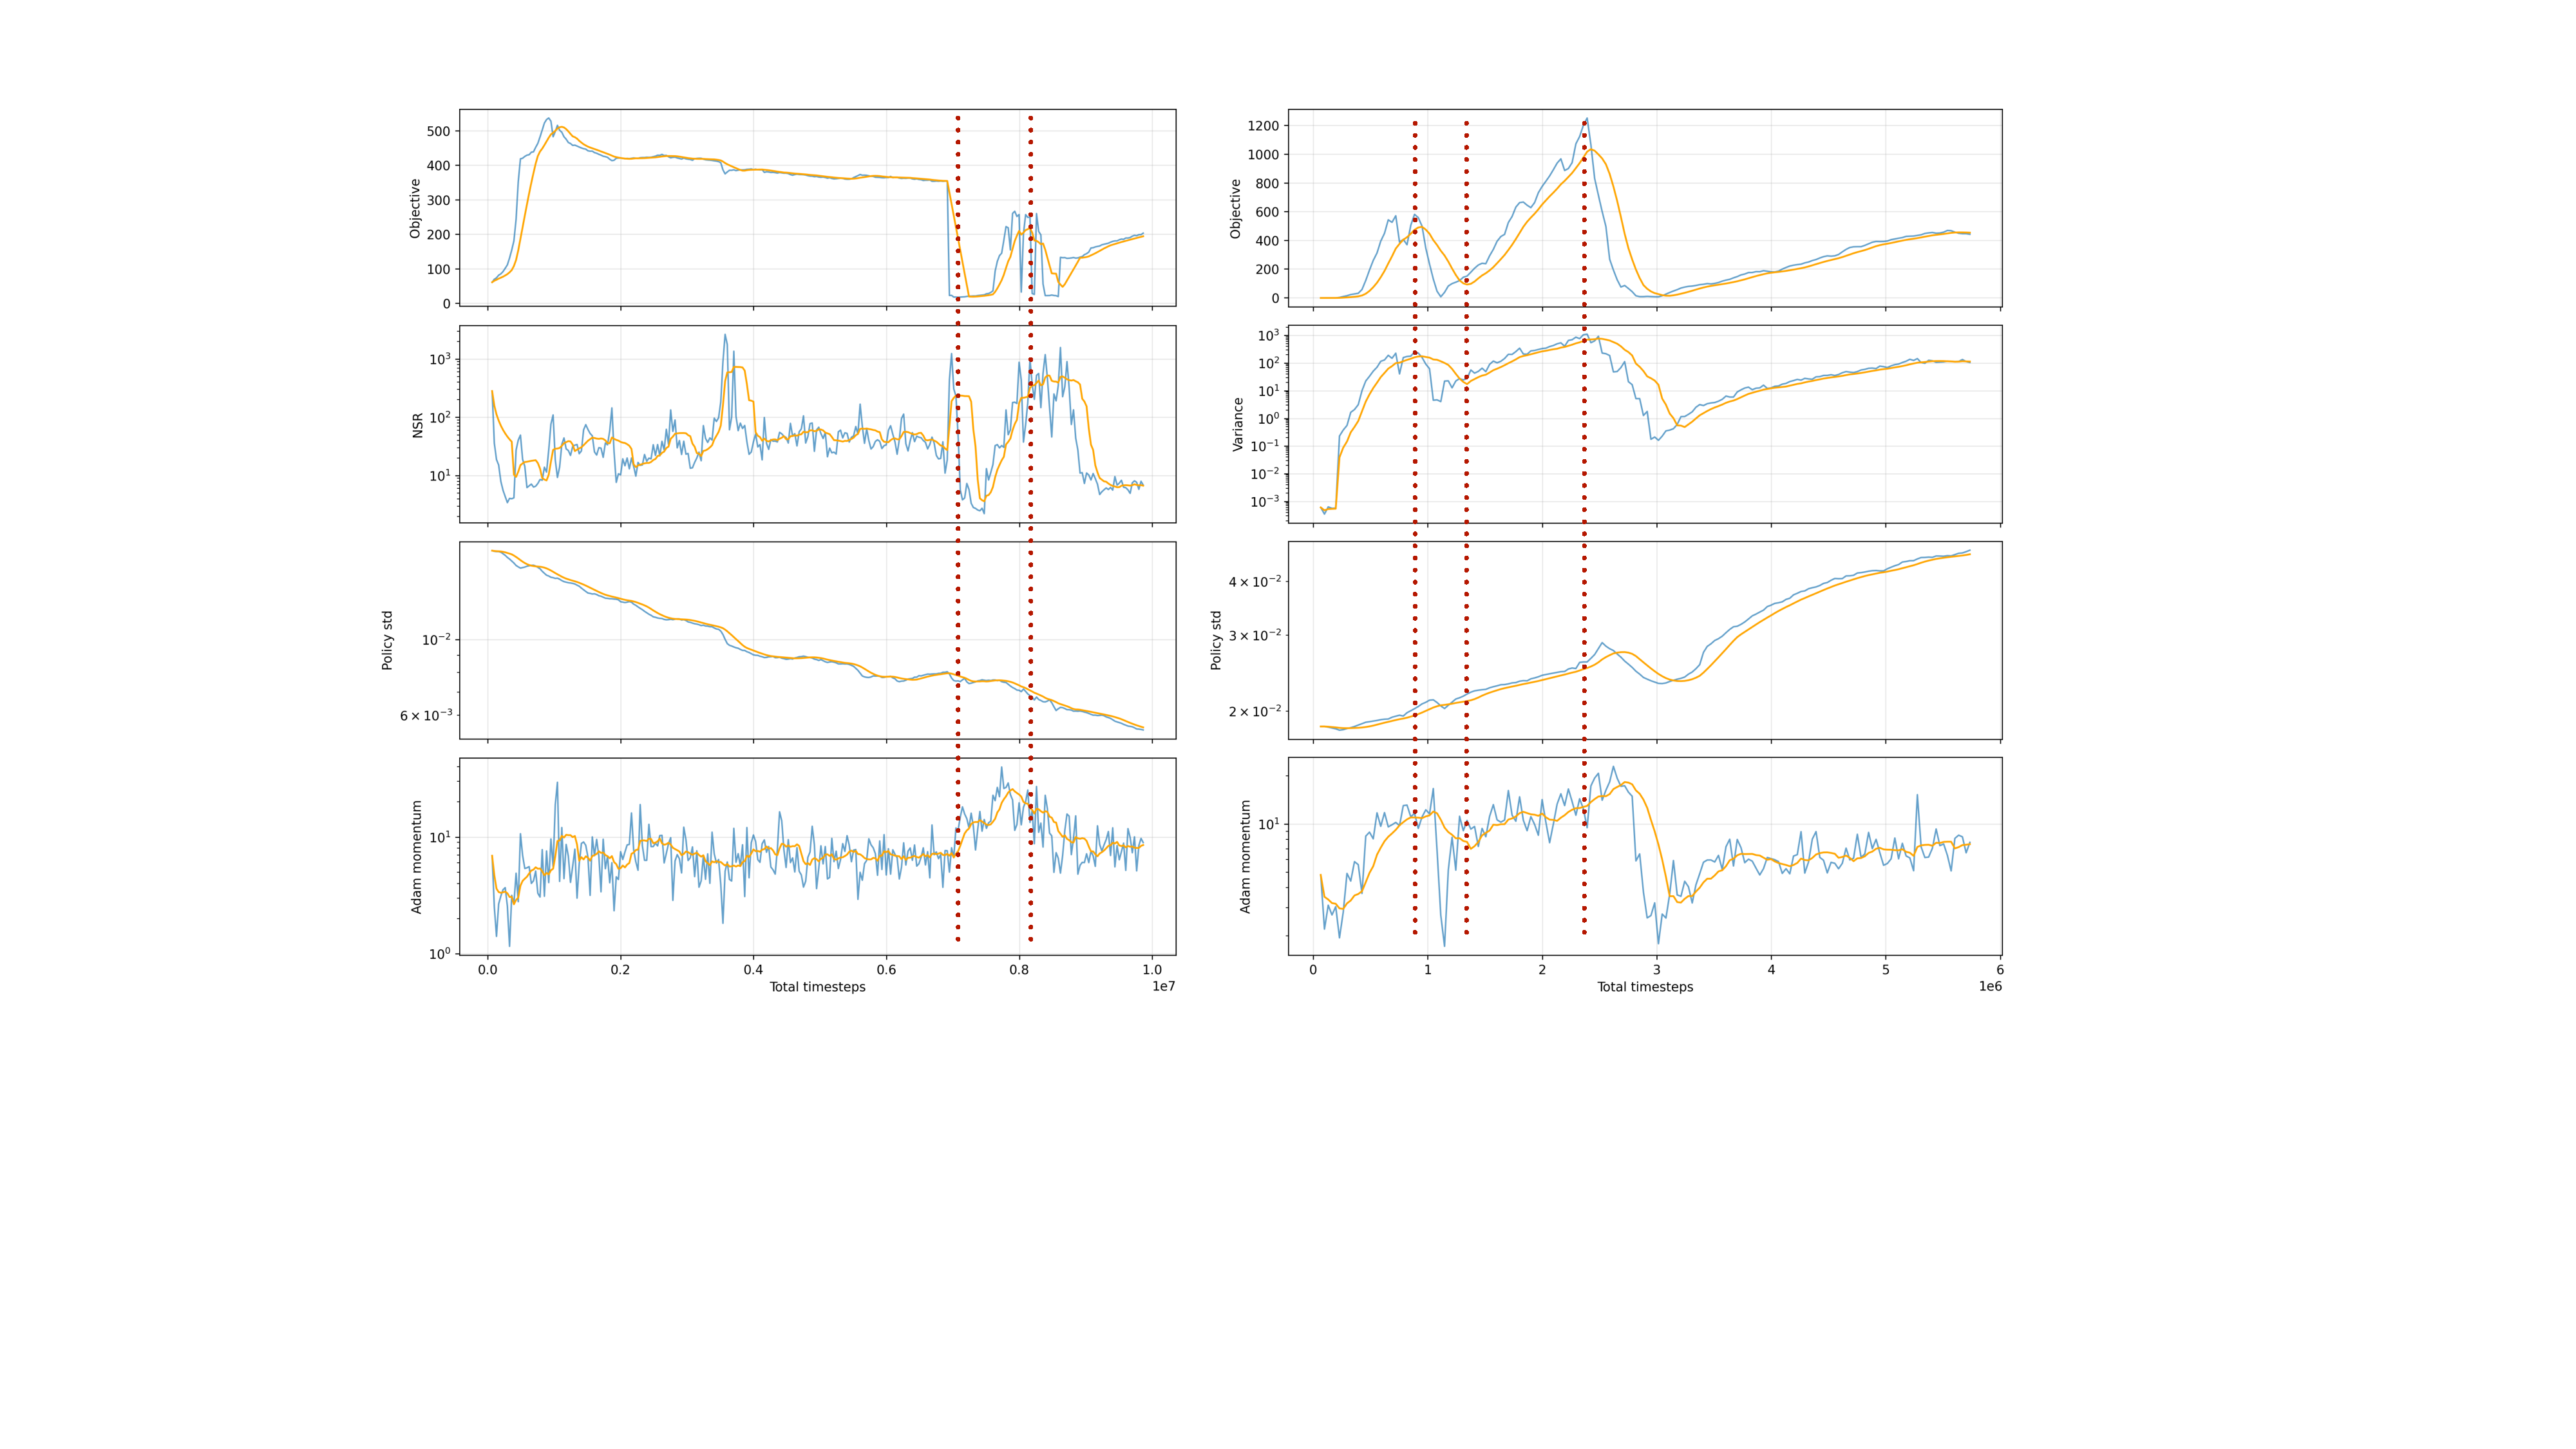
\includegraphics[width=0.9\textwidth]{figure/mujoco_collapse.pdf}
    \caption{MuJoCo experiments that show instability caused by large NSR. Left: Hopper-v4 environment; Right: HalfCheetah-v4 environment. From top to bottom we show the objective, the NSR, the log standard deviation of the policy covariance, and Adam's momentum. Red dashed lines show the synchronized fluctuations in objective and NSR.}
    \label{fig:mujoco_collapse}
\end{figure}
